\documentclass[11pt]{article}
\usepackage{graphicx}
\usepackage{float}

\begin{document}

\title{The Crane Problem}
\author{Ivan Almer and Mislav Krstulović}

\maketitle

\section{Problem Statement}

\subsection{Backstory}
On a sunny day in Cartagena (Spain) my friend Mislav and me were chilling on the rooftop of our apartment overlooking the nearby mountains. Next to us, there was a moving crane which led us to a discussion whether it is possible that, looking at the crane from above, the load carried by the crane always has the linear path from some starting point to its destination.
This motivated us to further define the problem and already seemed like it had the potential for some mental gymnastics.

\begin{figure}[H]
\centering
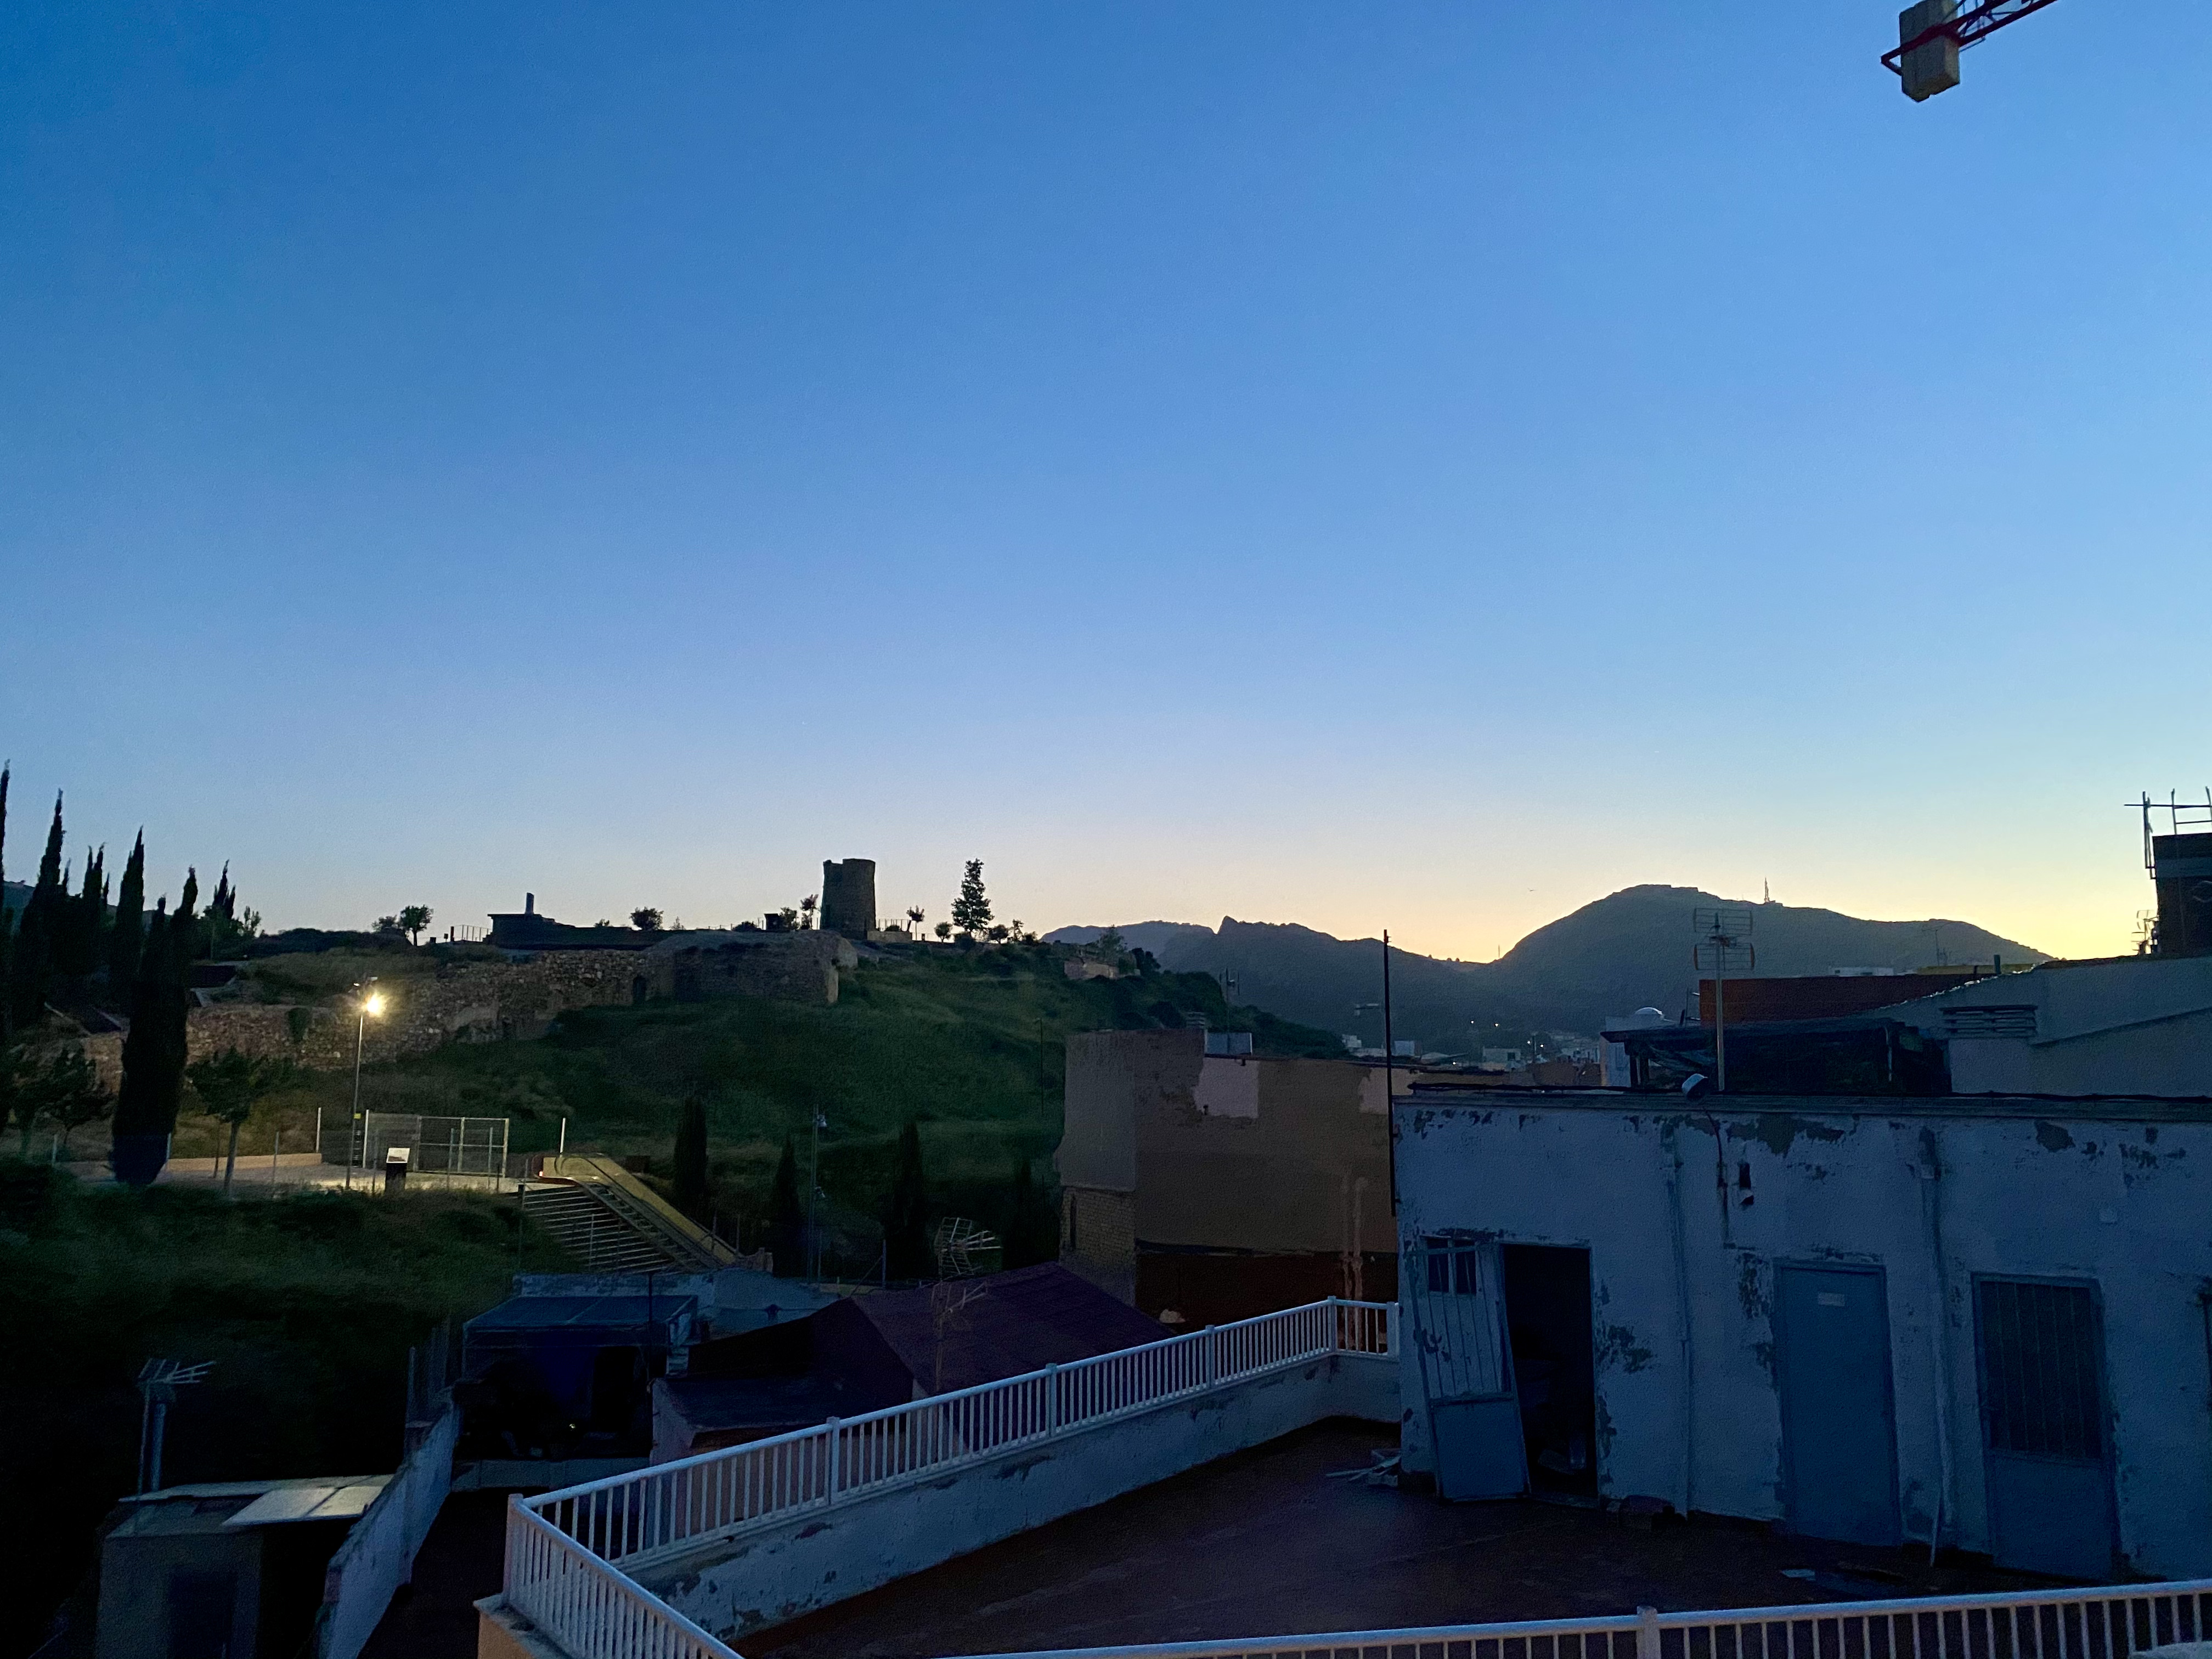
\includegraphics[width=10cm]{rooftop.jpeg}
\caption{Rooftop where the idea came to be}\label{fig:rooftop}
\end{figure}

\subsection{Problem}
Suppose we have a load located at the starting location $S = (s_1,s_2)$ and its destination is the ending point $E = (e_1,e_2)$. The crane rotates at a constant angular velocity $\omega$ and starts rotating at time $t=0$ to the side of our choosing. The load carried by the crane can move along the arm of the crane and the speed along the arm is $c(t)$:

\begin{figure}[H]
\centering
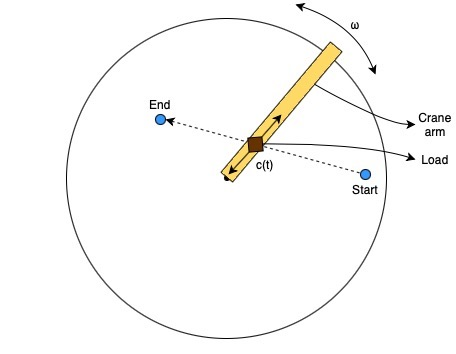
\includegraphics[width=10cm]{crane.jpg}
\caption{Crane - view from above}
\label{fig:crane}
\end{figure}

At the time $t=0$ the load is located at the starting point and the crane immediately starts rotating such that it covers the smaller angle between starting and ending point. For example in the image above, the crane will rotate in the counterclockwise direction because both $S$ and $E$ are on the upper half of the circle. Had $E$ been in the lower half, the crane would start rotating in the clockwise direction. \\

\textbf{Problem:} Find the function $c(t)$ such that the load always has a linear trajectory from the start to the end (dashed line on the image above). For this problem, there are no restrictions for the function $c(t)$ (such as maximum velocity or similar).

\section{Solution}

We will restrict ourselves to the case when the starting point $S$ is on the positive side of $x$-axis ($\varphi = 0$), like on the figure \ref{fig:crane}, because if that is not the case, it is possible to rotate the whole system so the point $S$ ends up at positive side $x$-axis. Moreover, when the system is rotated and the point $S$ is on $\varphi = 0$, if the ending point $E$ has the angle $\varphi > \pi$ we can just change the crane's rotation direction: $\varphi(t) = -\omega t$. If the ending point has $\varphi < \pi$ then the rotation direction stays positive: $\varphi(t) = \omega t$.\\

Having said this, the further derivation of the formula will only focus on the positive rotation, because the problem can always be mirrored around the $x$-axis such that the rotation is positive.\\

We can decompose the velocity of the load into 2 independent velocities: the velocity of the load caused by the rotation of the arm of the crane and the velocity of the load along the arm of the crane. First let's formally write down the velocity caused by the rotation of the arm.\\

\subsection{Load velocity caused by the rotation}

\begin{figure}[H]
\centering
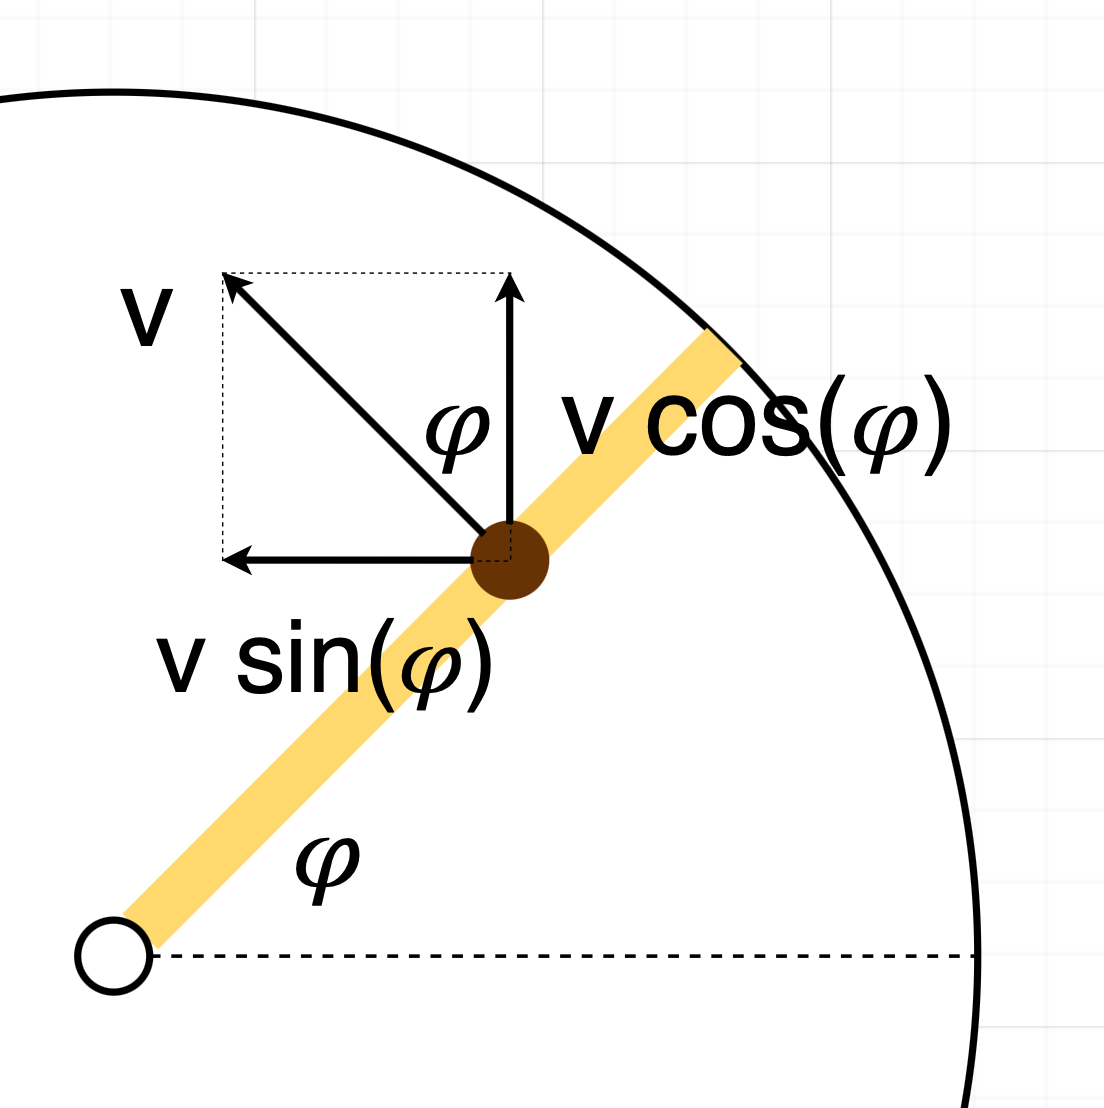
\includegraphics[width=6cm]{rotation_velocity.jpg}
\caption{Rotation velocity}
\label{fig:rot_velocity}
\end{figure}

Let's denote the rotation velocity $v_r$ of the load. When the radius is fixed and the load is moving at that velocity it covers the whole perimeter $2r\pi$ in time $\Delta t$. In that same time, $\Delta t$ the arm of the crane rotates fully around the center covering the angle of $2\pi$.

Which means we have the following: \( \omega = \frac{2\pi}{\Delta t} = const \), \( v_r = \frac{2r\pi}{\Delta t} \)\\

We deduct the formula for the amount of velocity at the distance from the center of the crane $r$:
\[ v_r = r\omega \]

Since this is only the length of the vector, we need to take care of the direction as well. Looking at the figure \ref{fig:rot_velocity} it is visible that the horizontal component of the velocity is equal to $-v_rsin(\varphi)$ and the vertical component is equal to $v_rcos(\varphi)$. Ultimately the vector of the velocity caused by the rotation of the arm is:

% \[ \vec{v_r}(\varphi) = (-v_r sin(\varphi), v_r cos(\varphi)) \]
\[ \vec{v_r}(t) = (-r(t)\omega sin(\varphi(t)), r\omega cos(\varphi(t))) \]

\subsection{Load velocity along the arm of the crane}

Finding the function of the velocity along the arm of the crane is the problem we need to solve. So we denote the velocity along the arm with $c(t)$, where the velocity is positive if the radius $r$ increases, and the negative if it decreases. The radius $r$ is obviously also dependant on $t$.

\[ c(t) = \frac{dr}{dt} \]

The $c(t)$ only denotes the length of the vector of velocity along the arm of the crane and we need to decompose that velocity into horizontal and vertical components.

\begin{figure}[H]
\centering
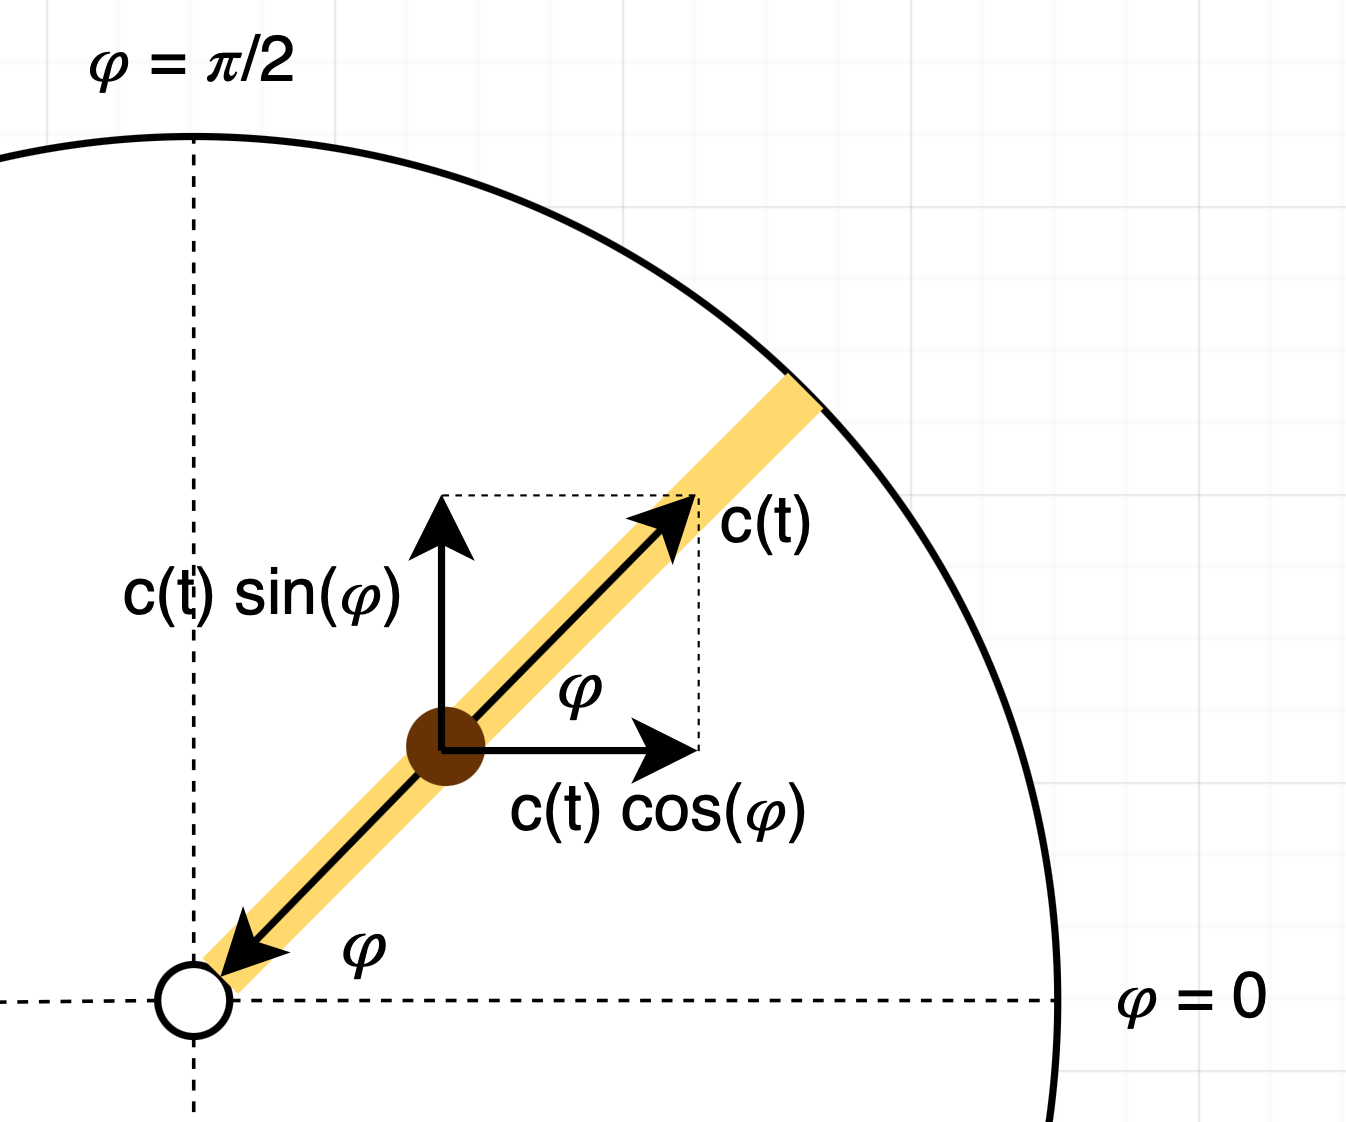
\includegraphics[width=6cm]{arm_velocity.jpg}
\caption{Velocity along the arm}
\label{fig:rot_velocity}
\end{figure}

\noindent From the figure above it is visible that the velocity along the arm $\vec{v_a}(t)$ is as follows:

\[ \vec{v_a}(t) = (c(t) cos(\varphi(t)), c(t) sin(\varphi(t))) \]

\subsection{Combining the two}

Now that we have both velocities defined and explicitly written, we can start finding the expression for $c(t)$. The resulting velocity will be:

\[ \vec{v_{tot}}(t) = (v_{totx}, v_{toty}) \]
\[ \vec{v_{tot}}(t) = \vec{v_a}(t) + \vec{v_r}(t) = (c(t) cos(\varphi(t)) - r(t)\omega sin(\varphi(t)), c(t) sin(\varphi(t)) + r(t)\omega cos(\varphi(t))) \]


The way to ensure that the load will have the linear path from point $S$ to point $E$ is that the total velocity vector always has the direction same as the vector connecting the two points. Let's denote that direction with $a$:

\[ a = \frac{e_2 - s_2}{e_1 - s_1} \]

\noindent and equalize that with the direction of the total velocity of the load:

\[ a = \frac{c(t)sin(\varphi(t)) + r(t)\omega cos(\varphi(t))}{c(t)cos(\varphi(t)) - r(t)\omega sin(\varphi(t))} \]

\[ a [c(t)cos(\varphi(t)) - r(t)\omega sin(\varphi(t))] = c(t)sin(\varphi(t)) + r(t)\omega cos(\varphi(t)) \]

\noindent we use the fact that the $c(t) = \frac{dr}{dt}$

\[ a\frac{dr}{dt}cos(\varphi(t)) - r(t)a\omega sin(\varphi(t)) = \frac{dr}{dt}sin(\varphi(t)) + r\omega cos(\varphi(t))\]

\[ \frac{dr}{dt}[a\cdot cos(\varphi(t)) - sin(\varphi(t))] = r\omega[cos(\varphi(t))+a\cdot sin(\varphi(t))] \]

\[ \frac{dr}{r} = \frac{a\cdot sin(\varphi(t))+cos(\varphi(t))}{a\cdot cos(\varphi(t))-sin(\varphi(t))}\omega dt \]

At this point, we will assume the positive rotation of the crane. This means that that $\varphi(t) = \omega t$ and that $d\varphi = \omega dt$. With that in mind, we continue with the derivation of the formula.

\[ \frac{dr}{r} = \frac{a\cdot sin(\varphi)+cos(\varphi)}{a\cdot cos(\varphi)-sin(\varphi)}d\varphi \]

% \int x^2 \,dx

\[ \int \frac{1}{r} \,dr = \int \frac{a\cdot sin(\varphi)+cos(\varphi)}{a\cdot cos(\varphi)-sin(\varphi)} \,d\varphi = \Bigg| \begin{array}{ll}
                  u = a\cdot cos(\varphi) - sin(\varphi)\\
                  du = -(a\cdot cos(\varphi) - sin(\varphi)d\varphi)
                \end{array}
                \Bigg|= - \int \frac{1}{u} \,du
\]

\[ \log{r} = -\log{u} + C_1 \ \ \ \Rightarrow \ \ \ \log{r} = -\log{(a\cdot cos(\varphi) - sin(\varphi))} + C_1\]
% \[ \log{r} = -\log{(a\cdot cos(\varphi) - sin(\varphi))} + C_1 \]

\[ r = \frac{C}{a\cdot cos(\varphi - sin(\varphi)(t)}\]
\[ r(t) = \frac{C}{a\cdot cos(\omega t) - sin(\omega t)}\]

To get rid of the constant and get the exact value, we need to take into account the starting condition. At the time $t=0$ the radius of the load was equal to the distance of the point $S$ from the center.

\[ r(0) = \sqrt{s_1^2 + s_2^2} = r_0 \]
\[ r(0) = \frac{C}{a\cdot 1 - 0} = r_0 \ \ \ \Rightarrow \ \ \ C = a\cdot r_0 \]

Now we have the expression for the radius of the load dependent on the time $t$:

\[ r(t) = \frac{a\cdot r_0}{a\cdot cos(\omega t) - sin(\omega t)}\]

To get the expression for the velocity $c(t)$ we can simply take the derivative of the radius:

\[ c(t) = \frac{dr}{dt} = -a\cdot r_0 \frac{-a\cdot sin(\omega t) - cos(\omega t)}{[a\cdot cos(\omega t) - sin(\omega t)]^2}\]

\[ c(t) = a\cdot r_0 \frac{a\cdot sin(\omega t) + cos(\omega t)}{[a\cdot cos(\omega t) - sin(\omega t)]^2} \]

That's it! :)

\end{document}
